\documentclass{article}
\usepackage[utf8]{inputenc}
\usepackage{amssymb}
\usepackage{tikz}
\usepackage{pgfplots}
\usepackage[letterpaper, margin=1.25in]{geometry}

\title{CS251 Midterm 1 - Fall 2022}
\author{schari}
\date{September 2022}

\begin{document}

\maketitle

\section{Summations and Logarithm Rules}
\begin{itemize}
    \item Summations
        \begin{itemize}
            \item Given $c$ is a constant, $\sum_{i = m}^{n} c = c(n - m + 1)$
            \item $\sum_{i = 1}^{n} i = \frac{1}{2}n(n + 1)$
            \item $\sum_{i = 1}^{n} i^2 = \frac{1}{6}n(n + 1)(2n + 1)$
            \item Given a function $f(i)$, $\sum_{i = m}^{n} f(i) = \sum_{i = 1}^{n} f(i) - \sum_{i = 1}^{m - 1} f(i)$
        \end{itemize}
    \item Log Rules
        \begin{itemize}
            \item In CS 251, if you are just given a $\log(n)$ without a base, they probably mean $\log_2(n)$
            \item $\log(ab) = \log(a) + \log(b)$
            \item $\log(\frac{a}{b}) = \log(a) - \log(b)$
            \item Given 2 numbers $a$ and $b$, $\log_a(n) = \frac{\log_b(n)}{\log_b(a)}$
            \item $\log(n^a) = a \log(n)$
            \item $a^{\log_a(n)} = n$
            \item $a^{b \log_a(n)} = n^b$
        \end{itemize}
\end{itemize}

\section{Experimental Analysis}

\begin{itemize}
    \item Limitations
        \begin{itemize}
                % Make these more concrete phrases instead of from the slides
            \item Different machines can vary the run time 
            \item other processes/noise
            \item May not be precise all the time 
        \end{itemize}
    \item These limitations are all put together to form constants $c$, which are seen in just about any runtime cost. In the power law, they are lumped together into a proportionality constant $a$.
    \item The power law is the law that $T(n)$ approximately follows the equation $T(n) = a * n^b$. The coefficient $a$ will be based on the hardware, which you cannot control. However, the value of $b$ is dependent on the algorithm.
    \item Given a table that contains data for $n$ and the associated $T(n)$'s, we can check if the data  follows the power law.
    \item Firstly, you can check if the values follow the power law by identifying the ratios between the rows of $T(n)$ and $n$. If the ratio between the rows of $n$ are consistent, then the ratios between the rows of $T(n)$ should also be consistent (though it can be a different ratio between $n$ and $T(n)$ and be okay. They just have to be consistent with their own rows).
        \begin{itemize}
            \item If the ratios between rows of $n$ are not consistent, that doesn't mean it doesn't follow the power law, only that its harder to check. Check the value of $\log_{r_n} (r_{T(n)})$ where $r_n$ is the ratio between two rows of $n$ and $r_{T(n)}$ is the ratio between rows of $T(n)$ (the same rows). For any two rows, this value should be essentially the same for it to follow the power law.
        \end{itemize}
    \item
        Another way of identifying if the values follow the power law is to create a log-log plot. Plot the values of $\log n$ and $\log T(n)$ on a plot and determine if they approximately make a straight line. If they do, they follow the power law.

        \begin{center}
            \begin{tikzpicture}[domain=0:3]
                \begin{axis}[xlabel={$\log n$}, ylabel={$\log T(n)$}]
                    \addplot[scatter, scatter src=\thisrow{class},
                    error bars/.cd, y dir=both, x dir=both, y explicit, x explicit, error bar style={color=mapped color}]
                    table[x=x,y=y] {
                        % The data here is absolutely garbage lol. Not at all from reality.
                        x       y        class
                        0.98521 1        0
                        0.49238 0.5      0
                        1.09346 1.111111 0
                        1.23021 1.25     0
                        1.40567 1.428571 0
                        1.63971 1.666667 0
                        1.96753 2        0
                    };
                \end{axis}
            \end{tikzpicture}
        \end{center}

    \item
        Once it is identified that data follows the power law, a prediction can be made. If the next value of $n$ given has the same ratio to a previous value, you can use the ratio of $T(n)$ to determine the predicted value of $T(n)$ very easily. 
        \begin{itemize}
            \item Given $T(8) = 16$ and $T(16) = 48$ and that $T(n)$ follows the power law, you can determine $T(64) = T(16 * 2^2) \approx T(16) * 3^2 = 48 * 9 = 432$ (The 2 and 3 are determined from the ratios, $16/8 = 2$ and $48/16$ = 3.)
        \end{itemize}
    \item
        You could be asked for the value of $b$ in $T(n) = a * n^b$. You can determine this via 
        \begin{enumerate}
            \item Determining the slope of the log-log plot. That value is $b$. 
            \item Take the logarithm of the ratio between rows of $T(n)$ with the base of the ratio of the rows of $n$. $b = \log_{r_n} (r_{T(n)})$.
                \begin{itemize}
                    \item For the given example of $T(8) = 16$ and $T(16) = 48$, $r_n = 16 / 8 = 2$ and $r_{T(n)} = 48 / 16 = 3$. Therefore, $b = \log_2 3$.
                \end{itemize}
        \end{enumerate}

\end{itemize}

\section{Recursive Functions}
\begin{itemize}
    \item Functions that call themselves in order to solve simpler problems
    \item Recursive functions don't call themselves infinitely; eventually stop when they reach a base case
    \item 
\end{itemize}

\section{Runtime Analysis}
\begin{itemize}
    \item Represents the efficiency of an algorithm
        \begin{itemize}
            \item Usually represents the cost of an algorithm for a specific value of n. 
            \item However, can be amortized if the cost is distributed over an interval of values of n. (Equation is $\sum_{k=a}^{b} T(k) / (b-a+1)$)
        \end{itemize}
    \item Three types of asymptotic runtime analysis: $O(n)$, $\Omega(n)$, and $\Theta(n)$
    \item $O(n)$
        \begin{itemize}
            \item The asymptotic upper bound
            \item Definition: Given functions $f(n)$ and $g(n)$, then $f(n) \in O(g(n))$ if there exists constants $c$ and $n_0$ where $0 \leq f(n) \leq cg(n)$ for all $n \geq n_0$
            \item In other words, $f(n) \in O(g(n))$ if $f(n)$ doesn't grow faster than $g(n)$.
            \item Growth order:
                \begin{itemize}
                    \item $O(1) < O(\log(n)) < O(n) < O(n \log(n)) < O(n^2) < O(n^3) < O(2^n) < O(n!)$
                \end{itemize}
            \item Going from the definition above, multiple functions can be big-$O$ of another function.
                \begin{itemize}
                    \item Ex: $n \in O(n)$, and $n \in O(n^2)$
                \end{itemize}
            \item Generally, if they're asking for big-$O$ of a function, you want to give the tightest bound of the function.
            \item When giving the $O(n)$ of a function, you take the fastest-growing term and remove the constants from it
                \begin{itemize}
                    \item Ex: $4n^2 + 2n\log(n) + 3n + 123456 \in O(n^2)$
                \end{itemize}
        \end{itemize}
    \item $\Omega(n)$
        \begin{itemize}
            \item Asymptotic lower bound
            \item Definition: Given functions $f(n)$ and $g(n)$, then $f(n) \in \Omega(g(n))$ if there exists constants $c$ and $n_0$ where $0 \leq cg(n) \leq f(n)$ for all $n \geq n_0$
            \item In other words, $f(n) \in \Omega(g(n))$ if $f(n)$ doesn't grow slower than $g(n)$.
            \item Like how multiple functions can be $O(n)$ of a function, multiple functions can also be $\Omega(n)$ of a function
                \begin{itemize}
                    \item Ex: $n \in \Omega(n)$, and $n \in \Omega(\log(n))$
                \end{itemize}
            \item Again, generally you should give the tightest bound
            \item Process for getting big-$\Omega$ of a function is same as getting big-$O$
        \end{itemize}
    \item $\Theta(n)$
        \begin{itemize}
            \item Asymptotic tightest bound of a function
            \item $f(n) \in \Theta(g(n))$ if $f(n)$ doesn't grow faster or slower than $g(n)$
        \end{itemize}
    \item Asymptotic Growth Properties
        \begin{itemize}
            \item If $f(n) \in O(g(n))$ and $f(n) \in \Omega(g(n))$, then $f(n) \in \Omega(g(n))$ and vice versa
            \item If $f(n) \in O(g(n))$ and $g(n) \in O(h(n))$, then $f(n) \in O(h(n))$
            \item If $f(n) \in \Omega(g(n))$ and $g(n) \in \Omega(h(n))$, then $f(n) \in \Omega(h(n))$
            \item If $f(n) \in \Theta(g(n))$ and $g(n) \in \Theta(h(n))$, then $f(n) \in \Theta(h(n))$
            \item If $f(n) \in O(h(n))$ and $g(n) \in O(h(n))$, then $f(n) + g(n) \in O(h(n))$
            \item If $f(n) \in \Theta(g(n))$, then $f(n) + g(n) \in \Theta(g(n))$
            \item If $f(n) \in O(g(n))$, then $g(n) \in \Omega(f(n))$
        \end{itemize}
\end{itemize}


\section{Algorithm Analysis}
\begin{itemize}
    \item Given an algorithm, we need to find the runtime cost of it.
    \item The runtime cost is based on what is specifically deemed worthy of noting. This can be the following:
        \begin{itemize}
            \item The number of iterations.
                \begin{itemize}
                    \item for$(i = 0; i < n; i++) // $Do something
                \end{itemize}
            \item The value of a variable
                \begin{itemize}
                    \item 
                        $total = 0;$

                        for$(i = 0; i < n; i++)$ $total += i$
                \end{itemize}
            \item The number of times a function is ran.
                \begin{itemize}
                    \item for$(i = 0; i < n; i++) f(i)$ where $f(i)$ has a undefined cost correlating to the arguments.
                \end{itemize}
            \item The summed cost of function calls based on the arguments of the function.
                \begin{itemize}
                    \item for$(i = 0; i < n; i++) f(i)$ where $f(i)$ has a defined cost (e.g. $f(i) = i$ or $f(i) = \log i$).
                \end{itemize}
        \end{itemize}
    \item Some rules that you can follow are the following:
        \begin{itemize}
            \item
                Loops and recursion generally turn into sigma notation.
            \item
                If there is an "if" statement or other condition, it is usually better to seperate it into seperate parts or entire equations, instead of trying to keep it in the same parts. This includes things like the base case of a recursive function, if the base case counts as an iteration!
            \item
                If the loop is going backwards, you can turn it around if it makes it easier. (e.g. you can turn subtraction into addition and swap upper and lower bounds, or division to multiplication), Just be careful its still the same iteration values!
            \item
                If the comparison "$< f(n)$" is used, you probably want to use "ceil(f(n)) - 1" ($\lceil f(n) \rceil - 1$) as the upper bound. If its "$<= f(n)$", you probably want "floor(f(n))" ($\lfloor f(n) \rfloor$)
            \item
                However, if looking at an asymptotic cost ($O(n)$, $\Omega(n)$, $\Theta(n)$), then you probably don't need floor and ceil at all, because they are miniscule compared to the entire sum.
        \end{itemize}
    \item There are a number of ways of taking an algorithm and determining the cost.
        \begin{itemize}
            \item
                Given a loop where a variable is incremented by 1 between each iteration, a simple sigma notation can be used.

                for$(i = 0; i < n; i++) f(i) \Rightarrow$
                $\sum_{i=0}^{n-1} T_f(i)$
            \item
                Given a loop where a variable is multiplied by c between each iteration, you can use log, and then replace any value of $i$ with $2^k$.

                for$(i = 1; i < n; i *= c) f(i) \Rightarrow$
                $\sum_{k=0}^{\lceil \log_c n \rceil - 1} T_f(2^k)$
            \item
                Given a recursive function that takes an input $n$, with base case $a$, and does a $f(n)$ cost operation, and then runs itself with value $n-1$, the summation would be:
                $\sum_{k=a}^{n} f(k)$

                Notice that this is exactly the same as a loop. For basic recursive functions, they are basically just loops. Anything else you might want induction.
            \item
                This is something we haven't covered, but it is useful in some circumstances.
                Given a loop where a variable is incremented by k between each iteration, you can stretch or squish the sigma accordingly.

                for$(i = a; i < n; i += k) f(i) \Rightarrow$
                $\sum_{i=0}^{\lceil(n-a)/k \rceil - 1} T_f(ki + a)$
        \end{itemize}
\end{itemize}


\section{Arrays and LinkedLists}
\begin{itemize}
    \item Arrays
        \begin{itemize}
            \item A fixed size sequential data structure
            \item Accessing data in an array $\in O(1)$
            \item Inserting an element at the end of the array
                \begin{itemize}
                    \item If you keep track of the next available cell, $O(1)$
                    \item If not, $O(n)$
                \end{itemize}
            \item Inserting an element in the middle of a sorted array
                \begin{itemize}
                    \item Determining the position to insert the element + shifting elements to the right: $O(n)$
                \end{itemize}
            \item Resizing an array
                \begin{itemize}
                    \item Increasing the size of an array involves creating a new array with a larger size, then transferring the elements from the array to the new array
                    \item This process is $T(n) \approx n \in O(n)$
                    \item In order to minimize the amount of times we have to repeat the process of expanding the array, we generally double the size of the old array
                    \item Because this resizing is done so infrequently, we \textit{amortize} this operation; that is, average it over several elements. Essentially, because we don't resize this array when inserting the first $n$ elements, when the $n + 1^{\mathrm{th}}$ element is inserted, despite resizing the array being relatively costly, we do it infrequently enough so that the average runtime cost is not as extreme.
                    \item Example proof: Let $T(k)$ be the runtime cost associated with resizing the array when inserting $k$ elements into an array of size $n$. This means that the amortized cost $T(n) = \sum_{k = 1}^{n + 1} \frac{1}{n + 1}T(k)$. \\

                        When $k \leq n$, we do not resize the array, since the array still has capacity to accept new elements. Therefore, when $k \leq n$, $T(k) = 0$ since nothing is done to expand the array. Meanwhile, when $k = n + 1$, because we are resizing the array, we incur the full cost from resizing the array. Therefore, $T(n + 1) = n$. \\

                        Therefore,
                        $$\sum_{k = 1}^{n + 1} \frac{1}{n + 1}T(k) = \frac{1}{n + 1}(0 + 0 + \ldots + 0 + n) =$$
                        $$ \frac{n}{n + 1} = 1 - \frac{1}{n + 1} \in O(1)$$

                        Therefore, the amortized runtime of $T(n) \in O(1)$.
                    \item Here, I'm justifying why $T(k)$ evaluates the way it does at various values, then I'm taking the average of $T(k)$ at the various values I've specified.
                \end{itemize}
        \end{itemize}
    \item LinkedLists
        \begin{itemize}
            \item A dynamic linear data structure
            \item There are a few kinds of linked lists
                \begin{itemize}
                    \item Singly linked lists: each node in the list points to the next element in the list
                    \item Doubly linked list: each node in the list points to the next and previous element in the list
                    \item Circularly linked list: the last element in the list points to the first (and in a doubly circular linked list, the first element will point to the last element)
                \end{itemize}
            \item Accessing data in an array $\in O(n)$
                \begin{itemize}
                    \item This is because you will have to traverse through the list to get to the item you are accessing
                \end{itemize}
            \item Inserting an element into the list
                \begin{itemize}
                    \item Inserting at the front of the list $\in O(1)$
                    \item Inserting at the back of the list:
                        \begin{itemize}
                            \item If you have a pointer to the end of the list: $\in O(1)$
                            \item If not, $\in O(n)$
                        \end{itemize}
                    \item Inserting in the middle of the list: $\in O(n)$
                \end{itemize}
            \item Deleting an element from the list
                \begin{itemize}
                    \item Singly linked list $\in O(n)$ since you have to always loop from the front
                    \item Doubly linked list $\in O(1)$ since you can also loop from the rear and save time then
                \end{itemize}
        \end{itemize}
    \item \underline{Pros} vs \textit{Cons} of Arrays and LinkedLists
        \begin{itemize}
            \item Arrays: \underline{direct access to any element in the array}, \underline{no pointers}, \textit{is fixed in size}, \textit{requires consecutive space in memory to initialize}
            \item LinkedLists: \underline{Resizeable}, \underline{easy insertion at the front or back of the list}, \textit{space overhead because of pointers}, \textit{cannot easily access an element in the middle of the list}
        \end{itemize}
\end{itemize}

\section{Stacks}
\begin{itemize}
    \item Data structure to store and remove data
    \item Last data pushed into the stack would be the first data popped off (LIFO)
        \begin{itemize}
            \item Think of it like a stack of plates; the last plate placed on top is the first plate taken from the stack
        \end{itemize}
    \item Standard methods for stacks:
        \begin{itemize}
            \item \verb|push()| - Add an element to the top of the stack
            \item \verb|pop()| - Remove the element from the top of the stack
            \item \verb|isEmpty()| - Whether or not there are elements on the stock
            \item \verb|size()| - Number of elements on the stack
            \item \verb|peek()| - View the element at the top of the stack without removing it
        \end{itemize}
    \item Implementation using Arrays vs LinkedLists
        \begin{itemize}
            \item Arrays: Lower memory overhead; unable to resize to accomodate more elements
            \item LinkedLists: Pointers require more memory; can expand to increase number of elements in the stack
        \end{itemize}
\end{itemize}

\section{Queues}
\begin{itemize}
    \item Data structure to store and remove data
    \item First data enqueued would be the first data dequeued (FIFO)
        \begin{itemize}
            \item Think of it as a queue of people; first person to enter is also the first person who gets served
        \end{itemize}
    \item Standard methods for queues:
        \begin{itemize}
            \item \verb|enqueue()| - Add an element to the end of the queue
            \item \verb|dequeue()| - Remove the element from the front of the queue
            \item \verb|isEmpty()| - Whether or not there are elements in the queue
            \item \verb|size()| - Number of elements in the queue
            \item \verb|peek()| - View the element at the front of the queue without removing it
        \end{itemize}
    \item Implementation using Arrays vs LinkedLists
        \begin{itemize}
            \item Arrays: In addition to lower memory overhead, a queue implementation will loop from the end of array to the front, and will keep track of the index of the front and back of the queue (see slides for example).
            \item LinkedLists: Because LinkedLists are relatively resizable, you don't need to keep track of indices, but you will have to keep track of the front and back of the queue nodes.
        \end{itemize}
\end{itemize}

\section{Trees}
\begin{itemize}
    \item Non-linear, top-down structures
    \item Composed of a series of nodes that point to children (the node that points to children is called a parent)
    \item Trees can have 0 to many children
    \item Concepts:
        \begin{itemize}
            \item Size: number of nodes in Trees
            \item A tree is empty when it has 0 nodes in it
            \item Root: Node that has no parent nodes
            \item Parent: Node that points to this node
            \item Grandparent: Node that points to parent node
            \item Sibling: nodes besides current node that parent node points to
            \item Children: Nodes that current node points to
            \item Leaf: Node that has no children
            \item Height: distance between lowest node and root node (root is height 0)
            \item Depth: same as height
        \end{itemize}
    \item Binary Trees
        \begin{itemize}
            \item Special kind of tree where each node has either 0, 1, or 2 children
            \item Designate these children as left or right
            \item Full binary tree: Every node has 2 children except for the leaves
            \item Complete binary tree: Except for leaves, the rest of the tree is a full binary tree. The leaves are inserted from left to right at the bottom.
            \item Properties of binary trees
                \begin{itemize}
                    \item Given a binary tree of height $h$, the maximum number of leaves it can have is $2^h$, and the maximum total number of nodes it can have is $2^{h + 1} - 1$
                \end{itemize}
            \item Traversing Binary Trees
                \begin{itemize}
                    \item We will use this tree as an example:

                        \begin{tikzpicture}
                            \node {A}
                            child{node [xshift = -0.5 cm]{B}
                            child{node {D}}
                            child{node {E}}}
                            child{node [xshift = 0.5 cm]{C}
                            child{node {F}}
                            child{node {G}}};
                        \end{tikzpicture}
                    \item Preorder
                        \begin{itemize}
                            \item Visit a node before its descendants (NLR)
                            \item Traversal thru current tree: A, B, D, E, C, F, G
                        \end{itemize}
                    \item Inorder
                        \begin{itemize}
                            \item Visit a node before its right descendant but after its left descendant (LNR)
                            \item Traversal thru current tree: D, B, E, A, F, C, G
                        \end{itemize}
                    \item Postorder
                        \begin{itemize}
                            \item Visit a node after its descendants (LRN)
                            \item Traversal thru current tree: D, E, B, F, C, G, A
                        \end{itemize}
                    \item Levels
                        \begin{itemize}
                            \item Traverse the tree one level at a time from left to right
                            \item Traversal thru current tree: A, B, C, D, E, F, G
                        \end{itemize}
                \end{itemize}
            \item Expression Trees
                \begin{itemize}
                    \item Can build binary trees out of arithmetic expressions by creating splits at significant operators
                    \item Example: Turning $x^2 + c = bx$ into an expression tree
                        \begin{enumerate}
                            \item Split at =

                                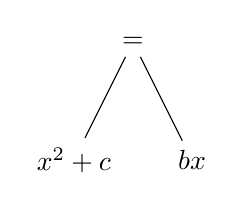
\begin{tikzpicture}
                                    \node {=}
                                    child{node {$x^2 + c$}}
                                    child{node {$bx$}};
                                \end{tikzpicture}
                            \item Split at +

                                \begin{tikzpicture}
                                    \node {=}
                                    child{node {+}
                                    child{node {$x^2$}}
                                    child{node {$c$}}}
                                    child{node {$bx$}};
                                \end{tikzpicture}
                            \item Split at $\times$

                                \begin{tikzpicture}
                                    \node {=}
                                    child{node [xshift = -0.5cm]{+}
                                    child{node {$x^2$}}
                                    child{node {$c$}}}
                                    child{node [xshift = 0.5cm]{$\times$}
                                    child{node {$b$}}
                                    child{node {$x$}}};
                                \end{tikzpicture}
                            \item Split at $\wedge$

                                \begin{tikzpicture}
                                    \node {=}
                                    child{node [xshift = -0.5cm]{+}
                                    child{node {$\wedge$}
                                    child{node {$x$}}
                                    child{node {$2$}}}
                                    child{node {$c$}}}
                                    child{node [xshift = 0.5cm]{$\times$}
                                    child{node {$b$}}
                                    child{node {$x$}}};
                                \end{tikzpicture}
                        \end{enumerate}
                    \item Order at which you split: $=, (), +-, \times/, \wedge$
                    \item You can also traverse these trees in the same way as other binary trees (preorder, inorder, postorder, levels).
                \end{itemize}
        \end{itemize}
    \end{itemize}

\end{document}

